\documentclass[12pt]{article}

\usepackage{xspace}
\usepackage{lineno}
\usepackage{setspace}
\usepackage{graphicx}
\usepackage{subfigure}
\usepackage{float}
\usepackage{color}
\usepackage{caption}
\usepackage[margin=1in]{geometry}
\usepackage{natbib}
\usepackage{amsmath}


\begin{document}
\doublespacing
\linenumbers

\newcommand{\kluyveri}{\textit{L. kluyveri}\xspace}


\noindent RH: LANDERER ET AL.--- Intragenomic variation in codon usage
% put in your own RH (running head)
% for POVs the RH is always POINT OF VIEW
\bigskip
\medskip
\begin{center}

% Insert your title:
\noindent{\Large \bf Differences in Codon Usage Bias between genomic regions in the yeast \textit{Lachancea kluyveri}.}
\bigskip

% We don't use a special title page; the author information is entered
% like any other text.

% FOOTNOTES: We don't allow them in the manuscript, except in
% tables. Don't include any footnotes in the text.


\noindent{C\textsc{EDRIC} ~{L\textsc{ANDERER}}$^{1,2,*}$,
R\textsc{USSELL} {Z\textsc{ARETZKI}}$^{3}$,
\textsc{AND}
M\textsc{ICHAEL} A.~{G\textsc{ILCHRIST}}$^{1,2}$}

\end{center}

\vfill

{\small
\noindent$^{1}$Department of Ecology \& Evolutionary Biology, University of Tennessee, Knoxville, TN 37996-1610\\
\noindent$^{2}$National Institute for Mathematical and Biological Synthesis, Knoxville, TN 37996-3410\\
\noindent$^{3}$Department of Business Analytics \& Statistics, Knoxville, TN ~ 37996-0532 \\
\noindent$^{*}$Corresponding author. E-mail:~cedric.landerer@gmail.com
}

\vfill
\centerline{Version dated: \today}
\vfill
\newpage


\begin{abstract}
Large efforts have been made to develop and explore models to understand intra-genomic variation in codon usage bias (CUB) and the contributions of mutation and selection to its evolution.
Comparative studies have been undertaken to further our understanding of variation in codon usage between species.
However, limited efforts have been made to understand how CUB is affected, and in return effects hybridization or introgression events between species with potentially large differences in CUB. 
In this study, we explore the CUB of \textit{Lachancea kluyveri} which has experienced a large introgression covering the whole left arm of chromosome C, affecting about 10\% of all genes.
The \kluyveri genome provides insights about the adaptation of introgressed regions to the novel genomic environment, with potentially large differences in selection for translation efficiency due to factors like tRNA availability, effective population size, or differences in mutation environment.

We analyzed the CUB of the endogenous \kluyveri genome and compared it to the CUB of the exogenous, introgressed region while separating the effects of mutation bias and selection for translation efficiency on CUB.
Our results show distinct CUB between the endogenous and exogenous regions of the \kluyveri genome.
We show that this differences can be mostly attributed to differences in mutation bias.

The introgression into the \kluyveri genome is of additional interest as the source has not yet been identified.
Given our ability to clearly distinguish CUB between the exogenous and the endogenous region we explored if CUB can identify possible candidates for the origin of the introgression.
The estimation of CUB and its separation into contributions of mutation and selection across a variety of yeasts allowed us to identify two candidates for the origin of the exogenous genes.
We used orthogonal information about synteny to validate candidates obtained by matching CUB.
\end{abstract}	



\section*{Outline}

\subsection*{Introduction}

\begin{itemize}
	\item CUB changes due to differences in mutation, selection, and drift.
	\item most studies assume only one environment for mutation, selection and drift and therefore only one codon usage.
	\begin{itemize}
		\item This assumptions can be violated for multiple reasons, like introgression/horizontal gene transfer (HGT), population bottlenecks, etc.
	\end{itemize}
	 \item Variation in CUB has previously only been studied in bacteria where HGT is common.
	\begin{itemize}
		\item HGT only transfers small amount of genes, probably with little to no impact on overall CUB.
		\item However, exogenous material can accumulate if HGT is frequent \citep{lawrence1997}.
		\item Previous studies have shown that genes with similar CUB are more likely to be transferred, potentially mitigating effects of accumulation \citep{tuller2011}.
		\item Hybridization/Introgression should have a larger impact on CUB due to the amount of material transferred, possibly affecting the outcome of a study if ignored. 
	\end{itemize}
	\item In this study, we look at \kluyveri (three key results).
	\begin{itemize}
		\item \kluyveri has experienced a recent ($55.5e10$ generations) large scale introgression \citep{friedrich2015}, clearly marked by elevated GC-content \citep{payen2009}.
		\item We expect that CUB differs between the introgressed exogenous region and the endogenous region due to the great ($13 \%$) difference in GC-content between the two regions.
		\begin{itemize}
			\item We find differences in CUB between the two regions.
			\item Taking this difference into account, we can increase our ability to extract biological information (predicting gene expression).
			\item Thanks to our ability to distinguish between effects of mutation and selection on CUB, we are able to attribute most of the difference in CUB to mutation bias.
			\item Figure \ref{fig:cub_all_aa} shows the CUB if we ignore the introgression (dotted), and for the endogenous (solid) and exogenous (dashed) respectively.
		\end{itemize}
		\item At this point, the source of the introgression has not been identified.
		\begin{itemize}
			\item Since we can clearly distinguish between the endogenous and exogenous CUB, can we use this information to find possible donor organisms?
			\item We analyzed CUB for several yeasts and found several species with similar selection for translation efficiency, and a few with similar mutation bias, but only two with high agreement in both (gossypii and dubliensis, Figure \ref{fig:corr_all_species}).
			\item We validated our findings with orthogonal information from synteny where analyzed a subset of our initial yeast set.
			\item We found several closely related species with syntenious regions, but only one species that also showed agreement in CUB allowing us to exclude dubliensis since it does not show any synteny with \kluyveri (Figure \ref{fig:synteny_species} right).
		\end{itemize}
		\item Assuming gossypii as origin for the exogenous region, we estimated a time since introgression from our estimates of mutation bias.
		\begin{itemize}
			\item Based on the two codon amino acids we estimated a time since introgression on the order of $10e8$
			\item We only used mutation bias as we would expect that differences in selection parameters would decay faster than in mutation.
			\item Assuming one to eight generations per day, we are finding an introgression age between 110k and 890k years, which overlaps with a previous estimate \citep{friedrich2015}.
		\end{itemize}
	\end{itemize}
\end{itemize}

\subsection*{Results}

\begin{itemize}
	\item We compared model fits of CUB for \kluyveri with a fit where we allowed CUB to vary between the endogenous and exogenous region.
	\begin{itemize}
		\item Model selection by AIC favored varying CUB between the endogenous and exogenous region of the \kluyveri genome.
		\item Comparison of predicted protein synthesis $\phi$ of both fits with empirical estimates showed that varying CUB improved our ability to predict $\phi$ ($0.59$ vs $0.69$) (Figure \ref{fig:phi_corr_two_cond}).
		\item We also observed a decrease of the variation in estimated $\phi$ when assuming only one CUB environment.
	\end{itemize}
	\item Comparison of posterior estimate between regions (Figure  \ref{fig:csp_comp}).
	\begin{itemize}
		\item We find that only 14 out of 40 $\Delta M$ parameters show the same sign, meaning that only $35 \%$ of $\Delta M$ agreed between regions (Figure \ref{fig:csp_comp}). 
		\item A closer look reveals that only two amino acids (A,F) favor the same codon by mutation in the two CUB environments.
		\item The comparison estimates of selection for translation inefficiency ($\Delta \eta$) showed that $30$ out of $40$ parameters ($75 \%$) showed the same sign, meaning that more of the same codons are favored by selection in both regions than in the mutation case (Figure \ref{fig:csp_comp}).
		\item We find that nine amino acids share a preferred codon.
	\end{itemize}
	\item The exogenous region is assumed to be a recent introgression of unknown origin \citep{friedrich2015}.
	\begin{itemize}
		\item To determine a potential origin, we estimated the number of neutral substitutions that we expect to determine how different we can the exogenous region to be from its origin.
		\begin{itemize}
			\item \citep{friedrich2015} argued that the introgression occurred about $55.5e6$ generations ago, and showed that it can be found in all studied populations.
			\item Based on the length of the exogenous region ($1e6$), the mutation rate per nucleotide ($4e-10$) and the number of generations estimated ($55.5e6$) we expect about $22k$ neutral substitutions or about $2.2 \%$ of the introgressed region.
		\end{itemize}
		\item Estimates of gene trees with a fixed topology allowed us to determine that we do not observe accelerated evolution in the exogenous region when compared to the endogenous region (Figure \ref{fig:rate_evol}).
		\item these observations combined lead us to the expectation that the exogenous region should still reflect most of its original CUB environment.
	\end{itemize}
	\item We explored CUB for several yeasts species to determine if another yeast shows similar CUB.
	\begin{itemize}
		\item Comparison of CUB parameters yielded three species with agreement ($\rho > 0.5$) in mutation bias ($\Delta M$) and $29$ species with agreement in selection bias ($\Delta \eta$) (Figure \ref{fig:corr_all_species}).
		\item Only two species, gossypii and dubliensis showed agreement in both, $\Delta M$ and $\Delta \eta$ (Figure \ref{fig:corr_all_species}).
		\item musiva showed a positive correlation in in both $\Delta M$ and $\Delta \eta$ but did not satisfy our arbitrary cutoff.
	\end{itemize}
	\item We used synteny as an independent approach as a means to validate our candidate list.
	\begin{itemize}
	\item We analyzed synteny relation between the introgression and species closely related to our two candidates and \kluyveri.
	\item The check revealed eight species (Figure \ref{fig:synteny_species}).
		\begin{itemize}
			\item dubliensis, a candidate based on CUB, did not show a synteny relationship with the exogenous region.
			\item gossypii, the other candidate, was found to have a synteny coverage of $95 \%$ (Figure \ref{fig:synteny_species}).
			\item the other six yeasts with synteny showed agreement with only agreement in $\Delta \eta$ but not in $\Delta M$ (CHECK mutation/selection CORRELATION for each species with synteny).
		\end{itemize}	 
	\end{itemize}
	\item Under the assumption that the exogenous region originated from gossypii, we estimated the time since introgression.
	\begin{itemize}
		\item For simplicity, only the two codon amino acids were used. 
		\item We again assumed a mutation rate of $4e-10$.
		\item Based on the difference in mutation bias $\Delta M$ between gossypii and the endogenous region we estimated a decay curve.
		\item knowing the current $\Delta M$ parameters allowed us to place the exogenous region on that curve, providing us with an estimate of the time since introgression of about $2.17e8$ generations.
		\item Two of the ten amino showed a negative time since introgression (K, N) without them, our estimate of the time since introgression changes to $3.06e8$.
		\item Assuming one to eight generations per day for \kluyveri we estimate a time since introgression of about $110k$-$890k$ (Table \ref{tab:intro_age})
		\item combining our estimates with the estimates of \citep{friedrich2015} ($19k$-$150k$) we date the age of the introgression to be between $110k$-$150k$.
		\item Our time since introgression depends on gossypii being the origin and has not changed it's CUB since the introgression occurred.
	\end{itemize}
\end{itemize}


\subsection*{Discussion}

\begin{itemize}
	\item Partitioning \kluyveri based on the the previously identified introgression allowed us to identify two distinct signatures of CUB.
	\begin{itemize}
		\item We find that while the endogenous region shows mutation bias towards T and A ending codons for many amino acids, the exogenous region is mutational biased towards C and G ending codons for many amino acids (only A,F share the same mutational favored codon, C,D,E,G,H,I,K,L,N,P,Q,R,S,T,V,Y,Z do not) (Figure \ref{fig:cub_all_aa}).
		\item While we find higher correlation between $\Delta \eta$ in both environments, most amino acids do not share their optimal codon (D,Y,N,H,I,K,P,S,T,V) (Figure \ref{fig:cub_all_aa}).
		\item We find that this is due to the preferred and the second codon switching places (S,T,V);  switching between C and T ending codons.
		\item Ignoring the difference in CUB environment between endogenous and exogenous region can lead to miss-classification of the preferred codon (CHECK how many AA disagree between full genome and endogenous).
		\item Furthermore, the high correlation between selection environments could have lead most approaches purely focused on selection to not only miss identify the preferred amino acid, but missed this interesting biology all together.
		\begin{itemize}
			\item While in this particular case GC-content provided an indication that CUB between endogenous and exogenous genes may differ, this indication moight not only be the case.
			\item We find many different CUB in the yeasts explored in this study and most of them have similar amounts of GC-content.
		\end{itemize}
		\item Separating CUB environments also allows us improve our ability to predict protein synthesis rate $\phi$.
		\begin{itemize}
			\item We can observe an interesting interplay between codon specific parameters ($\Delta M$ and $\Delta \eta$) and the gene specific parameter $\phi$, potentially serving as an indicator in the future when other indicators such as GC-content are lacking.
			\item When highlighting endogenous and exogenous genes in the full genome fit (Figure \ref{fig:phi_corr_two_cond} left) we observe that these genes are separating by $\phi$.
			\item This causes $\Delta M$ to be mostly informed by exogenous genes and $\Delta \eta$ to be mostly informed by endogenous genes (add suppl. fig. of correlation?).
			\item The higher agreement between selection parameters indicates that mostly effects on mutation have been miss-identified, but not only (see switching of preferred codon).
			\item We also observe that the variation in predicted $\phi$ is decreased if we ignore the differing CUB environments, likely as a results to accommodate two different CUB environments;
		\end{itemize}
	\end{itemize}
	\item The source of the introgression has not yet been identified.
	\begin{itemize}
		\item We expected differences in selection to decay faster, finding greater differences in mutation bias providing more information about the introgression; This is exactly what we find.
		\item However, it is likely that this is not as initially expected due to faster decay of differences in selection parameter.
		\begin{itemize}
			\item We find evidence (few substitutions expected, no elevated rate of evolution in the exogenous genes) that the introgressed region had experienced a similar selection on translation efficiency as \kluyveri.
			\item However, we are unable to conclusively show that the similarity is due to similarity between \kluyveri and the donor of the exogenous region and and due to decay.
		\end{itemize}
		\item The introgression is expected to have occurred recently and we have already established that we do not expect a lot of substitutions to have occurred.
		\begin{itemize}
			\item This lead us to hypothesize that the exogenous region should still show CUB similar to it's donor species.
			\item Providing us with the opportunity to explore if CUB can be used as a more fine grain (relative to GC-content) approach to scan for potential donor species.
		\end{itemize}
		\item The estimation of CUB parameters for several closely related yeast species revealed multiple 29 species that have a similar selective CUB component but only two with a similar mutation component.
		\begin{itemize}
			\item Mutation bias is more informative but not because it would decay slower as originally expected but because most yeast species explored have a similar selective environment.
			\item This shows that the information about the mutation component in CUB disregarded by other approaches like CAI provides valuable information about the evolution of CUB and should not be ignored.
		\end{itemize}
		\item The check for synteny revealed eight species, all within the Saccharomycetaceae group.
		\begin{itemize}
			\item Similarity CUB is therefore more widespread (broader in tree, not more frequent) than synteny as dubliensis which is not a Saccharomycetaceae shows a similar CUB.
			\item CUB in exogenous region and gossypii, and dubliensis may have evolved independently and could be due to an environmental responds (out of scope?) 
		\end{itemize} 
		\item In summary, using selection for translation efficiency allowed us to select 29 species as potential origin, adding mutation bias reduced this number to two, and in an effort to validate our findings using synteny we were able to reduce our candidate pool to one, gossypii. 
		\begin{itemize}
			\item In this particular case, with a small set of species and a strong signature of GC-content we would have been able to select gossypii as possible donor right away.
			\item (The next to points is how I would like to end this section but I am not sure how to do that)
			\item But it was never the point to actually identify the origin of the introgression and we have only provided a potential donor.
			\item It is more important that we applied what we learned about CUB evolution.
		\end{itemize}
	\end{itemize}
	\item Assuming gossypii as origin, we explored how fast mutation bias would decay if a region would be transferred between gossypii and \kluyveri and where the exogenous region fit along this timeline.
	\begin{itemize}
		\item The mutation rate we assumed is in line with other estimates of mutation in yeast (order of $1e-10$).
		\item The usage of two codon amino acids was for the sake of simplicity (think of better reason so reviewers won't ask for other AA). 
		\item While the decay rate for all amino acids was the same, due to the shared mutation rate employed, we find great variation in the estimate of the age of the introgression.
		\begin{itemize}
			\item Our approach assumes that gossypii has not evolved since the transfer of the exogenous region to \kluyveri.
			\item Finding two amino acids with a negative estimated introgression time indicate that this assumption is violated.
			\item If the exogenous region truly originated from gossypii, we can assume that the time since introgression is actually more recent than our estimate, bringing it closer to the estimate of \citep{friedrich2015}.
		\end{itemize}
	\end{itemize}	
	\item In conclusion, this study shows three things:
	\begin{itemize}
		\item More than one CUB environment can be present in a genome, due to introgression, or other, internal factors; and ignoring it can lead to misinterpretation of results.
		\item It is well established that CUB is driven by Mutation, Selection, and Drift; Here we illustrate again that it is important to utilize all three factors to gain a complete picture.
		\item While we used CUB to determine a potential origin of the exogenous region, this is just an example using the better understanding of CUB evolution we gained in this study.
	\end{itemize}
\end{itemize}


\bibliographystyle{plain}
\bibliography{kluyveri_paper}

\section*{Figures and Tables}

\begin{figure}[H]
    \centering
    \begin{subfigure}
        \centering
        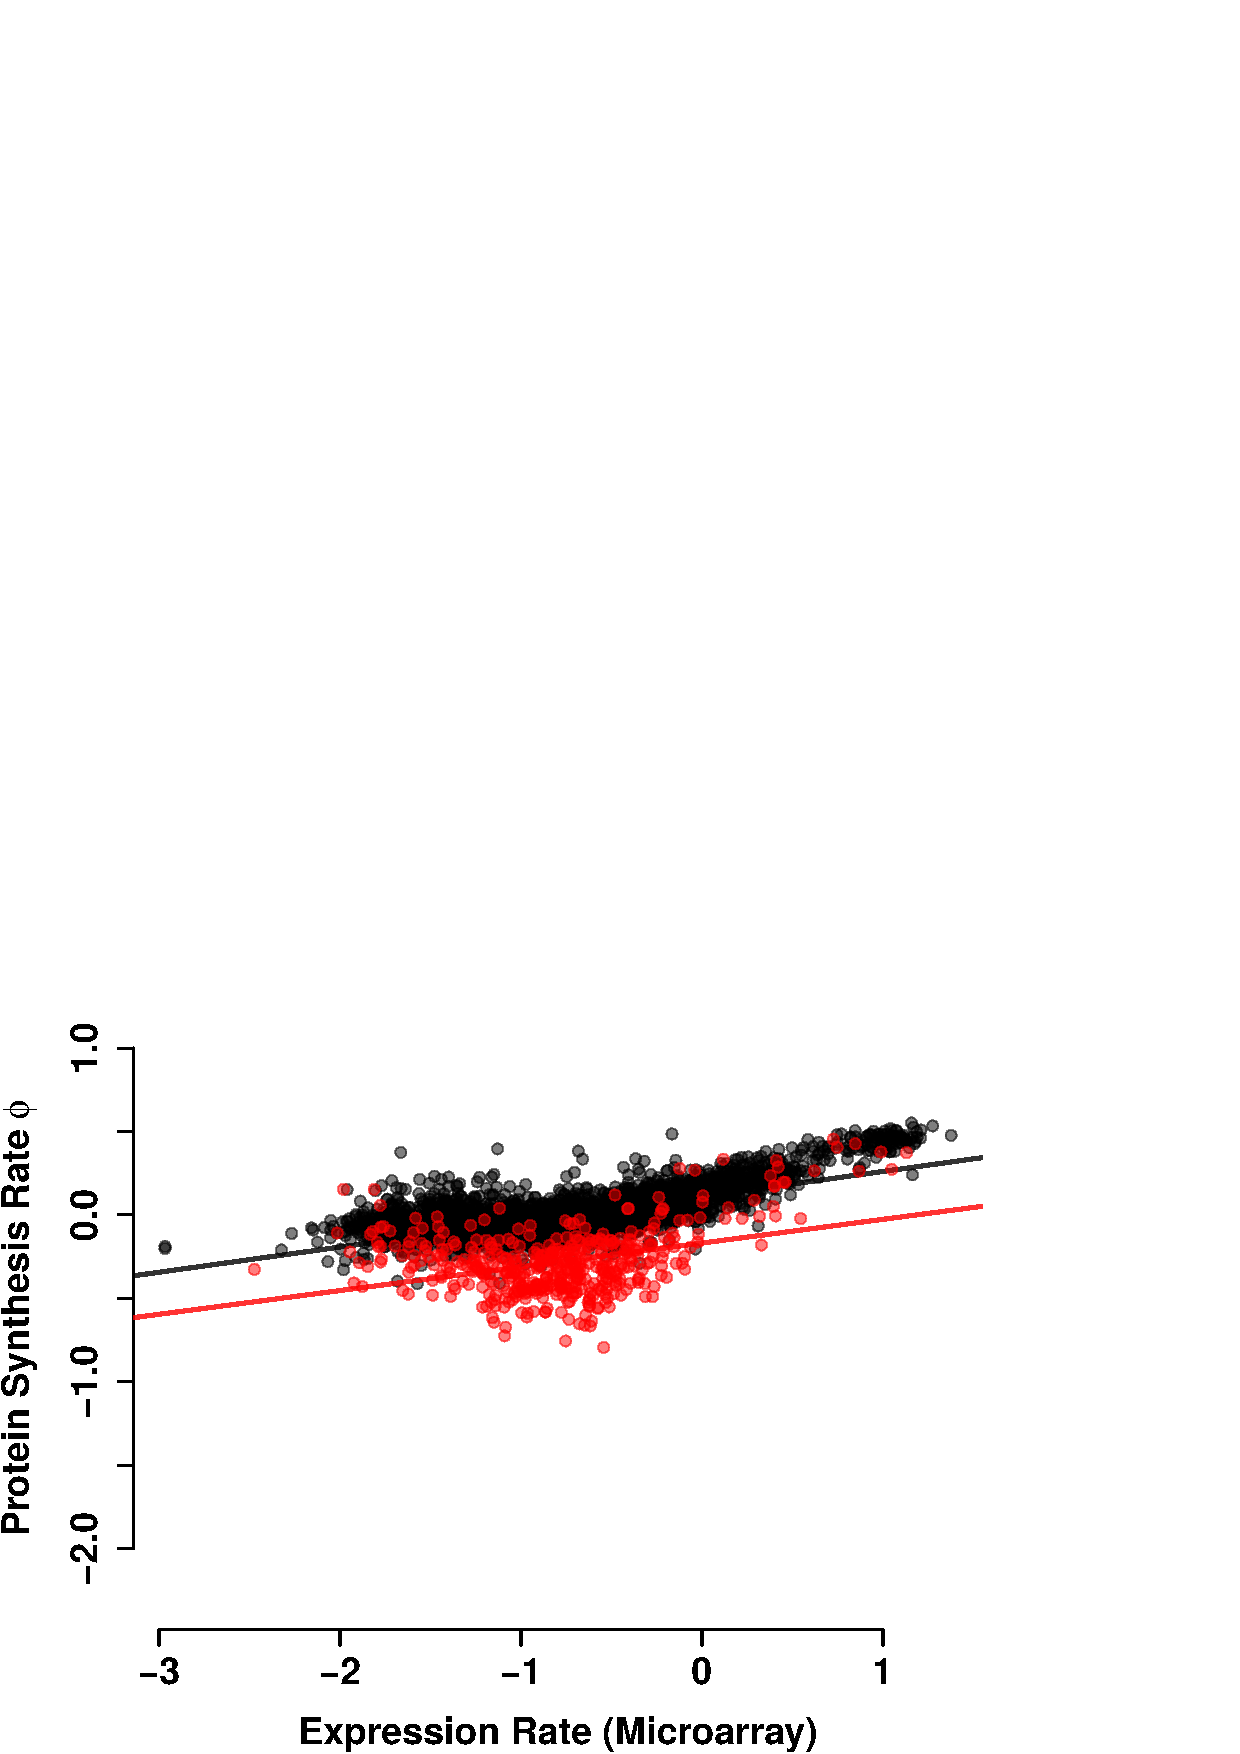
\includegraphics[width=.45\textwidth]{img/phi_corr_plot_whole_Genome_estim.pdf}
    \end{subfigure}
    \begin{subfigure}
        \centering
        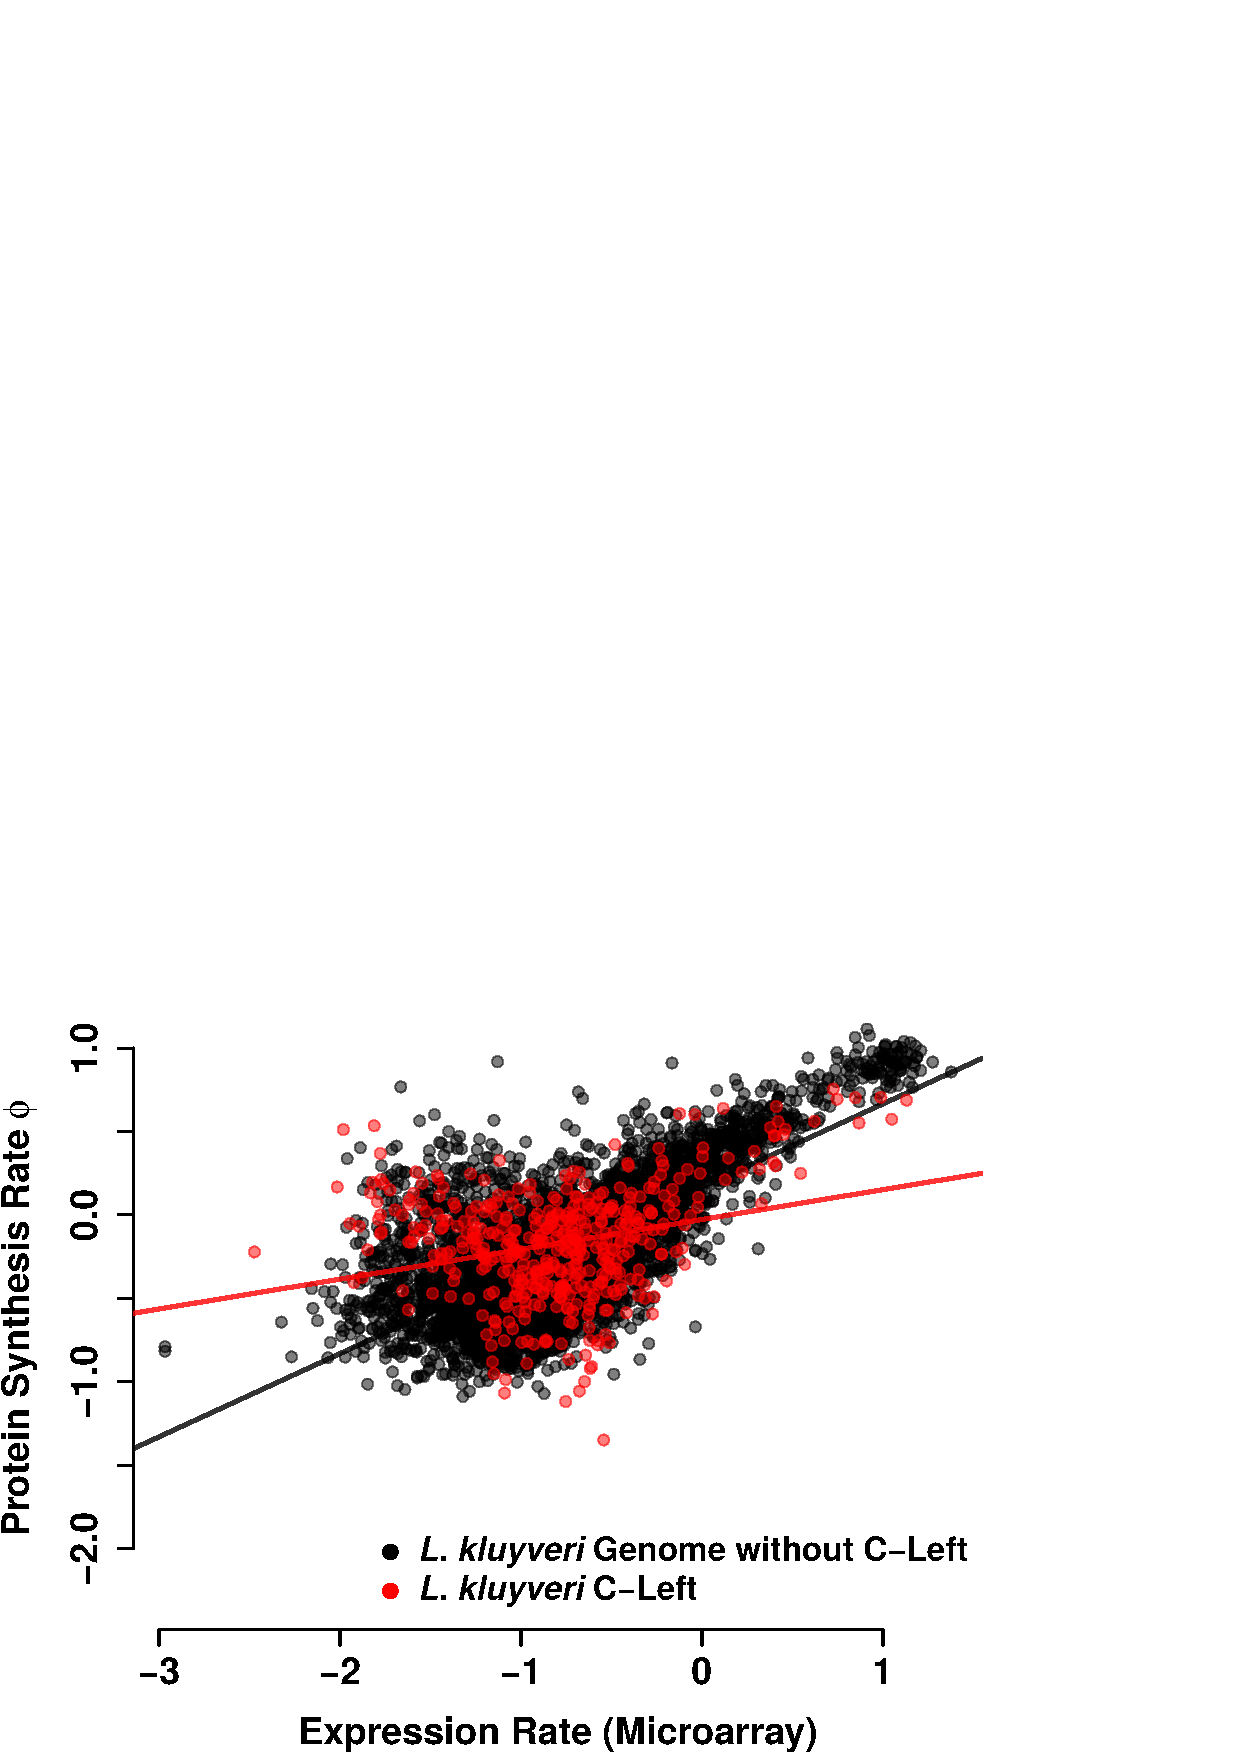
\includegraphics[width=.45\textwidth]{img/phi_corr_plot_split_Genome_estim.pdf}
    \end{subfigure}
    \caption{Person correlation of predicted protein synthesis rate $\phi$ with observed expression rate}
    \label{fig:phi_corr_two_cond}
\end{figure}

\begin{figure}[H]
    \centering
    \begin{subfigure}
        \centering
        \includegraphics[width=.45\textwidth]{img/csp_corr_dm.pdf}
    \end{subfigure}
    \begin{subfigure}
        \centering
        \includegraphics[width=.45\textwidth]{img/csp_corr_deta.pdf}
    \end{subfigure}
    \caption{Person correlation CUB parameters estimated from endogenous and exogenous genes}
    \label{fig:csp_comp}
\end{figure}

\begin{figure}[H]
     \centering
	\includegraphics[width=\textwidth]{img/CUB_cleft_main.pdf}
	\caption{Codon Usage. Modify figure to indicate whether same AA is optimal in endogenous/exogenous region? }
	\label{fig:cub_all_aa}
\end{figure}

\begin{figure}[H]
     \centering
	\includegraphics[width=\textwidth]{img/rate_of_evolution.pdf}
	\caption{Overall time passed along gene tree}
	\label{fig:rate_evol}
\end{figure}

\begin{figure}[H]
     \centering
	\includegraphics[width=\textwidth]{img/csp_correlations.pdf}
	\caption{Codon Usage}
	\label{fig:corr_all_species}
\end{figure}


\begin{figure}[H]
    \centering
    \begin{subfigure}
        \centering
        \includegraphics[width=.45\textwidth]{img/synteny_blocks_and_gc.pdf}
    \end{subfigure}
    \begin{subfigure}
        \centering
        \includegraphics[width=.45\textwidth]{img/synteny_coverage.pdf}
    \end{subfigure}
    \caption{Synteny stuff}
    \label{fig:synteny_species}
\end{figure}


\begin{table}
\centering
\begin{tabular}{ | c | c | c | c | c | c | }
\hline
	Codon & Amino Acid & $\Delta M_{Egos}$ & $\Delta M_{Endo}$ & $\Delta M_{Exo}$ & Generations \\ \hline
	TGC & Cys (C) & -3.28 & 0.20 & -1.34 & $4.81e8$ \\ \hline
	GAC & Asp (D) & -2.57 & 0.58 & -1.26  & $1.99e8$ \\ \hline
	GAA & Glu (E) & 2.47 & 0.45 & 1.26 & $6.30e8$ \\ \hline
	TTC & Phe (F) & -1.46 & 0.66 & 0.14  & $1.19e8$ \\ \hline
	CAC & His (H) & -2.31 & 0.48 & -1.37  & $2.49e8$ \\ \hline
	AAA & Lys (K) & 0.96 & -0.53 & 0.99 & $-2.78e7$ \\ \hline
	AAC & Asn (N) & -1.28 & 0.25 & -1.88 & $-2.54e8$ \\ \hline
	CAA & Gln (Q) & 2.98 & -0.25 & 1.67 & $3.57e8$ \\ \hline
	TAC & Tyr (Y) & -1.92 & 0.17 & -1.65 & $1.00e8$ \\ \hline
	AGC & Ser$_2 $ (Z) & -3.11 & 0.18 & -1.68 & $3.13e8$ \\ \hline
	& & & & &    \\ \hline
	& & & & Mean: & $2.17e8$ ($3.06e8$) \\ \hline
	& & & & Std Error: & $7.99e7$ ($6.41e7$) \\ \hline
\end{tabular}
\caption{Mutation rate is $3.8e-10$ (Lang 2008)}
\label{tab:intro_age}
\end{table}


\end{document}








